\documentclass[pdf]{beamer}
\usetheme{default} 

% Load packages
% Reference
\usepackage[style=apa]{biblatex}
\addbibresource{../references.bib}

% Caption
\usepackage{caption}
%\captionsetup[figure]{labelformat=empty} % Removes the label

% smileys
\usepackage{wasysym}

% Automatically create a section page at the beginning of each section
\AtBeginSection[]
{
    \begin{frame}
    \vfill
    \centering
    \begin{beamercolorbox}[sep=8pt,center,shadow=true,rounded=true]{title}
        \usebeamerfont{title}\insertsectionhead\par%
    \end{beamercolorbox}
    \vfill
    \end{frame}
}

%% preamble
\title{The Art of Positivity in Drawing: Unveiling the Impact of Positive Mood States on Visual Creativity via Deep Learning\vspace{1em}}
\subtitle{MACS 30200 Project}
\author{Sam Cong}
\institute{University of Chicago}
\date{\today}

\begin{document}
%% title frame
\begin{frame}
\titlepage
\end{frame}

% Table of Contents
% \begin{frame}
% \frametitle{Table of Contents}
% \tableofcontents
% \end{frame}

% Introduction Section
\section{Introduction}
\begin{frame}{Introduction}
\begin{itemize}
    \item<1-> \alert{Mood} pervades our entire framework of meaning, shaping our perception of the possibilities the world holds (\cite{ratcliffe_why_2013}).
    \item<1-> Positive emotions broaden thought-action repertoires (\cite{fredrickson_role_2001}).
    \item<2-> Speaking of thought-action repertoires, \alert{creativity} stands out as a fascinating human capacity to formulate novel ideas, methods, and solutions (\cite{hennessey_creativity_2010}).
    \item<3-> \textbf{How would positive moods influence creativity?}
\end{itemize}
\end{frame}

% {
% \setbeamercovered{transparent=10} % Set covered items to be semi-transparent
% \begin{frame}{Introduction}
% \begin{itemize}
%     \item<1> Mood pervades our entire framework of meaning, shaping our perception of the possibilities the world holds (\cite{ratcliffe_why_2013}).
%     \item<1> Positive emotions broaden thought-action repertoires (\cite{fredrickson_role_2001}).
%     \item<2> Speaking of thought-action repertoires, creativity stands out as a fascinating human capacity to formulate novel ideas, methods, and solutions (\cite{hennessey_creativity_2010}).
%     \item<3> How would positive moods influence creativity?
% \end{itemize}
% \end{frame}
% }

% Literature Review Section
\section{Literature Review}
\begin{frame}{The Psychology of Moods}
\begin{itemize} 
    \item<1-> Moods are diffuse affective states without a specific target and form the backdrop of our experiences (\cite{lischetzke_mood_2022}).
    % \item<2-> Moods develop more slowly while lasting longer than emotions and often from a combination of factors rather than specific events (\cite{desmet_15_2008}).
\end{itemize}
\end{frame}

\begin{frame}{The Psychology of Moods}
\begin{itemize}
    \item<1-> Multidimensional mood experiences (state-level mood) $=>$ \textcite{yik_structure_1999} proposed a unified framework of \alert{pleasant-unpleasant} and \alert{activated-deactivated} dimensions. 
    % \item<2-> A unified mood classification framework contributed to theory development on the cognitive and behavioral consequences of mood (\cite{lischetzke_mood_2022}):
    %     \begin{itemize}
    %         \item<3-> \textbf{Mood congruency} biases actions and processing (e.g., memory) towards events and influence strategies people use for mood regulation (\cite{larsen_toward_2000}).
    %         \item<4-> Moods affect general \textbf{information processing} (\cite{forgas_chapter_2017}):
    %             \begin{itemize}
    %                 \item<5-> Heuristic versus analytical processing (\cite{forgas_mood_1995});
    %                 \item<6-> Broadened versus narrowed attention spans;
    %                 \item<7-> Generosity of social judgments.
    %             \end{itemize}
    %     \end{itemize}
\end{itemize}
\end{frame}

% \begin{frame}{Demystifying creativity}
% \begin{itemize}
%     \item<1-> Influential \textit{standard} definition of creativity: ``generation of ideas, insights, or problem solutions that are new and meant to be useful'' (\cite[739]{de_dreu_hedonic_2008}).
%     \item<2-> Yet, this standard definition does not overshadow the \textbf{multiple dimensions of the construct of creativity}, e.g., cognitive, personal, developmental, social facets of creativity. 
% \end{itemize}
% \end{frame}

\begin{frame}{Demystifying creativity}
\begin{itemize}
    \item<1-> The cognitive aspect of creativity unravels the complexities of how creative ideas are formed and realized.
    \item<2-> Creativity as fundamental aspect of human cognitive abilities (\cite{ward_creative_1999}):
        \begin{itemize}
            \item<3-> Our versatile application of language;
            \item<4-> Our capability to form and apply new mental categories for organizing our experiences ...
            % \item<5-> Our skill in mentally handling objects ... 
        \end{itemize}
    % \item<2-> Theories transitioned from early, more mystical perceptions of creativity to acknowledging creativity as fundamental aspect of human cognitive abilities (\cite{ward_creative_1999}):
    %     \begin{itemize}
    %         \item<3-> Our versatile application of language;
    %         \item<4-> Our capability to form and apply new mental categories for organizing our experiences;
    %         \item<5-> Our skill in mentally handling objects ... 
    %     \end{itemize}
\end{itemize}
\end{frame}

\begin{frame}{Demystifying creativity}
\begin{itemize}
    \item<1-> Evolution of theoretical accounts to illuminate the cognitive systems underpinning creative thinking (\cite{johnson_divergent_2022}):
        \begin{itemize}
            \item<2-> \textbf{\textcite{mednick_associative_1962}'s Associative Theory} $=>$ The ability to form connections between distant concepts stored in memory;
            \item<3-> \textbf{\textcite{kaufman_cambridge_2010}'s Creative Cognition Approach} $=>$ Apart from basic cognitive operations such as attention and memory, knowledge (both \textit{depth} and \textit{breadth}) plays a crucial role in shaping creative thinking.
            \item<4-> \textbf{Theories on stage-like properties of creative processes} (e.g., \cite{finke_creative_1996}, \cite{patterson_personal_2004}) $=>$ 1) Generating ideas and later assessing their usefulness and suitability, 2) modifying them to achieve particular creative objectives.
        \end{itemize}
\end{itemize}
\end{frame}

\begin{frame}{Demystifying creativity}
An integrated framework: \textbf{Dual pathway to creativity model} (\cite{nijstad_dual_2010})
\begin{itemize}
    \item<1-> Identifies two primary pathways for creativity: \alert{cognitive flexibility} and \alert{cognitive persistence}:
        \begin{itemize}
            \item<2-> \textit{Cognitive flexibility}: switching between different perspectives, fostering the exploration of ideas and formation of novel connections, often enhanced by positive mood states.
            \item<3-> \textit{Cognitive persistence}: sustained and focused cognitive effort into a narrower set of ideas, typically enhanced by negative mood states that boost concentration and perseverance.
        \end{itemize}
\end{itemize}
\only<4->{
\begin{figure}
    \centering
    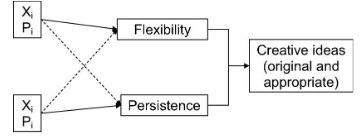
\includegraphics[height=0.2\textheight, keepaspectratio]{screenshots/Dual Pathway to Creativity Model.png}
    \caption{Dual Pathway to Creativity Model (\cite{nijstad_dual_2010})}
\end{figure}
}

\end{frame}

% \begin{frame}{Demystifying creativity}
% An integrated framework: \textbf{Dual pathway to creativity model} (\cite{nijstad_dual_2010})
% \begin{itemize}
%     \item <1-> Highlights the role of the prefrontal cortex, particularly the dorsolateral prefrontal cortex, in supporting creative cognitive activities through working memory and sustained attention.
%     \item <2-> Practical applications: Evaluating creativity in tasks using metrics such as \textit{fluency}, \textit{flexibility}, and \textit{originality}.
% \end{itemize}
% \end{frame}

% \begin{frame}{Mood-Creativity Linkage}
% \begin{itemize}
%     \item<1-> Previously conflicting findings on how different mood states influence creativity.
%     \item Potential reasons:
%         \begin{itemize}
%             \item<2-> Recall bipartite dimensions of mood states (\textit{valence} and \textit{activation} components);
%             \item<3-> Qualitative differences in different cognitive processes leading to creativity (e.g., \cite{finke_creative_1996}).
%         \end{itemize}
%     % \item<4-> Again, dual pathway to creativity model (\cite{nijstad_dual_2010}).
% \end{itemize}
% \end{frame}

\begin{frame}{Mood-Creativity Linkage}
\textbf{Dual pathway to creativity model} on mood-creativity linkage to reconcile previously conflicting findings on how different mood states influence creativity.
\end{frame}

\begin{frame}{Dual Pathway to Creativity Model on Mood-Creativity Link}
\begin{itemize}
    \item<1-> Mood influences creativity through \alert{two dimensions}: mood states (valence and activation) and their effects on cognitive pathways (flexibility and perseverance).
    \item<2-> \textbf{Positive hedonic tone} increases openness and receptiveness, enhancing flexibility, whereas \textbf{negative hedonic tone} leads to focused and deep task engagement, enhancing persistence.
    \item<3-> \textbf{Activating moods} (both positive and negative) are associated with increased energy and creativity. $=>$ Activating moods boost creative fluency and originality compared to deactivating moods (\cite{de_dreu_hedonic_2008}).
    \item<4-> \textbf{Positive activating moods} are linked to broader cognitive categories and faster completion times in creative tasks, while \textbf{negative activating moods} tend to generate more ideas within specific categories and involve longer completion times.
\end{itemize}
\end{frame}


\begin{frame}{Experimental Mood Induction}
\begin{itemize}
    \item<1-> One necessary condition to empirically test mood-creativity linkage is effectively inducing individuals’ mood changes.
    \vspace{1em}
    \item<2-> \smiley{} \alert{Experimental mood induction}: 1) effectiveness in altering mood (\cite{westermann_relative_1996}) and 2) causality evidence.
    % \vspace{1em}
    % \item<3-> \textcite{siedlecka_experimental_2019}'s classification framework for emotion induction methods: visual stimuli, music, imagery, autobiographical recall, and situational procedures.
    % \item<4-> Emotion induction techniques vary in effectiveness across the six basic emotions.
\end{itemize}
\end{frame}

% \begin{frame}{Experimental Mood Induction}
% \begin{itemize}
%     \item Emotion induction techniques vary in effectiveness across the six basic emotions (\cite{siedlecka_experimental_2019}):
%     \begin{enumerate}
%         \item Images or videos are effective for inducing a wide range of emotions;
%         \item Music strongly impacts emotions, especially happiness, fear, and sadness;
%         \item Recalling personal emotional experiences is effective for inducing anger, happiness, fear, disgust, and sadness, but less so for surprise ... 
%     \end{enumerate}
% \end{itemize}
% \end{frame}

\begin{frame}{Common Methods to Measure Creativity}
\begin{itemize}
    \item<1-> Another necessary condition to test mood-creativity linkage is choosing the appropriate method(s) to measure creativity.
    \item<2-> A diverse array of methodologies to assess the different facets of creativity (\cite{de_alencar_theory_2021}).
    \item<3-> \textbf{Development in creativity assessment} (\cite{kaufman_cambridge_2010}), including technology-based and ecologically valid assessments.
    % including psychometric tests, observational methods, self-assessment techniques, and naturalistic assessment. (\cite{kaufman_cambridge_2010}).
    % \item<3-> \textcite{batey_measurement_2012}'s 3-dimensional heuristic framework for creativity measurement:
    % \begin{figure}
    %     \centering
    %     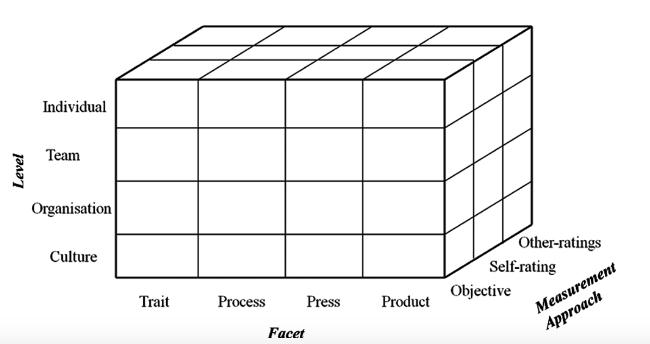
\includegraphics[height=0.4\textheight]{screenshots/Batey's new heuristic framework for creativity measurement.png}
    % \end{figure}
\end{itemize}
\end{frame}

\begin{frame}{Computational Approaches in Creativity Assessment}
\begin{itemize}
    \item<1-> \alert{Network science} $=>$ Modelling concept organization in semantic memory to test the associative theory of creativity (e.g., \cite{kenett_investigating_2014}, \cite{beaty_automating_2021});
    \item<2-> \alert{Deep learning \& computational linguistics} $=>$ E.g., text cohesion, readability, and meaningful psychological categories to measure creativity in creative writing (\cite{zedelius_beyond_2019}); automatic scoring originality of responses to divergent thinking tasks (\cite{patterson_multilingual_2023}).
\end{itemize}
\end{frame}

% \begin{frame}{Common Methods to Measure Creativity}
% \begin{itemize}
%     \item<1-> \textbf{Development in creativity assessment} (\cite{kaufman_cambridge_2010}), including refinement of traditional tests, introduction of technology-based assessments, and increasing emphasis on ecologically valid creativity assessment.
%     \item<2-> \textbf{Computational approaches} has been increasingly incorporated in creativity research:
%         \begin{itemize}
%             \item<3-> \alert{Network science} $=>$ Modelling concept organization in semantic memory to test the associative theory of creativity (e.g., \cite{kenett_investigating_2014}, \cite{beaty_automating_2021});
%             \item<4-> \alert{Deep learning \& computational linguistics} $=>$ E.g., text cohesion, readability, and meaningful psychological categories to measure creativity in creative writing (\cite{zedelius_beyond_2019}); automatic scoring originality of responses to divergent thinking tasks (\cite{patterson_multilingual_2023}).
%         \end{itemize}
% \end{itemize}
% \end{frame}

\begin{frame}{Common Methods to Measure Creativity}
Creativity research stands on the cusp of several promising developments in methodology (\cite{kaufman_cambridge_2010}):
\begin{itemize}
    \item Call for cross-disciplinary approaches.
    \item Effectively capture dynamics of (complex) creative processes;
\end{itemize}

\vspace{2em}
\begin{figure}
    \centering
    
\includegraphics{screenshots/Methodology.jpeg}
\end{figure}
\end{frame}

% Research Design Section
\section{Research Design}
\begin{frame}{Overview of Research Design}
\begin{itemize}
    \item<1-> \alert{Objective}: Join the debate on mood-creativity linkage using a) tasks that can track the dynamics of creative processes and b) novel methodologies from deep learning and NLP.
    \item<2-> Focus on positive mood varying on the \textit{activation} dimension: \textbf{happiness} (high activation) and \textbf{calmness} (low activation).
    \item<3-> Examine the \textit{flexibility} pathway (which links positive mood to creativity) proposed by the dual pathway to creativity model. 
    \vspace{2em}
    \only<4-> {
    \begin{figure}
        \centering
        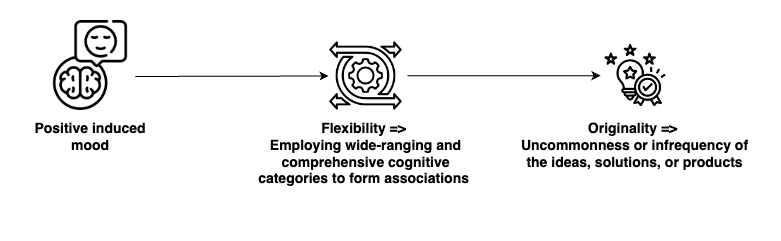
\includegraphics[width=\linewidth]{drawio/Overview of Research Design_Partial.png}
    \end{figure}
    }
\end{itemize}
\end{frame}

\begin{frame}{Overview of Research Design}
\begin{itemize}
    \item<1-> Follow \textcite{barbot_dynamics_2018}'s Multi-Trial Creative Ideation (MTCI) framework (featuring multi-stimuli approach \& dynamics of ideation process), use \textbf{incomplete shape drawing task} and \textbf{narrative about creative ideation processes} to track the dynamics of creative thinking.
    \only<1->{
    \begin{figure}
        \centering
        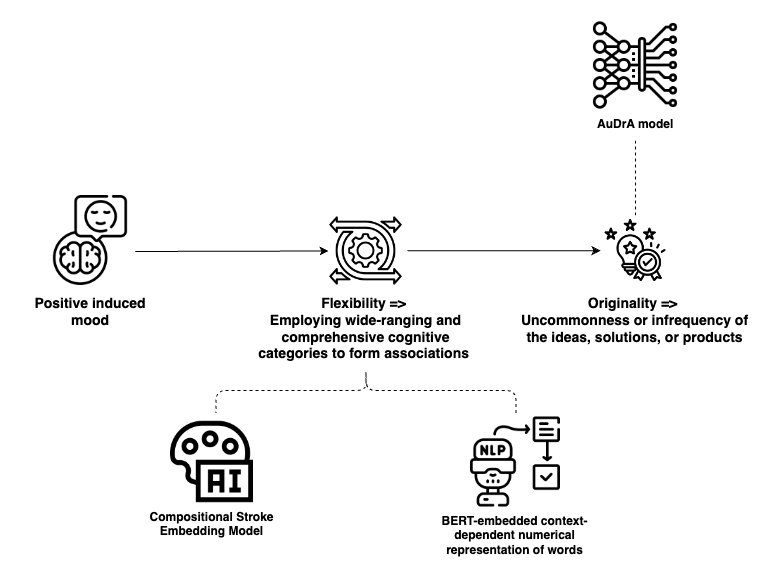
\includegraphics[height=0.6\textheight, width=0.85\textwidth]{drawio/Overview of Research Design_Full.png}
    \end{figure}
}
\end{itemize}
\end{frame}

{
\setbeamercovered{transparent=10} % Set covered items to be semi-transparent
\begin{frame}{Research Questions}
\begin{enumerate}
    \item<1> How do positive moods across the spectrum of activation level, including positive moods with high level of activation (e.g., happiness) and positive moods with low level of activation (e.g., calmness), affect (cognitive) flexibility during creative ideation process, respectively? 
    \item<2> How does (cognitive) flexibility during the creative ideation process further influence the originality aspect of creativity in the final product (i.e., whether flexibility mediates the relationship between positive mood and the originality aspect of creativity)?
\end{enumerate}
\end{frame}
}

\begin{frame}{Workflow}
\begin{figure}
    \centering
    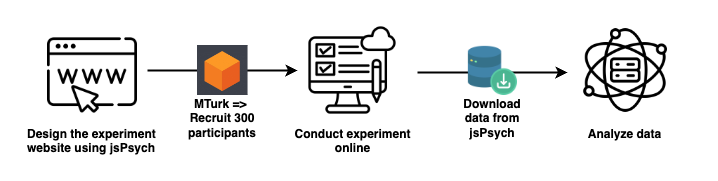
\includegraphics[width=\textwidth, keepaspectratio]{drawio/Workflow.png}
\end{figure}
\end{frame}

\begin{frame}{Experiment Timeline}
\begin{figure}
    \centering
    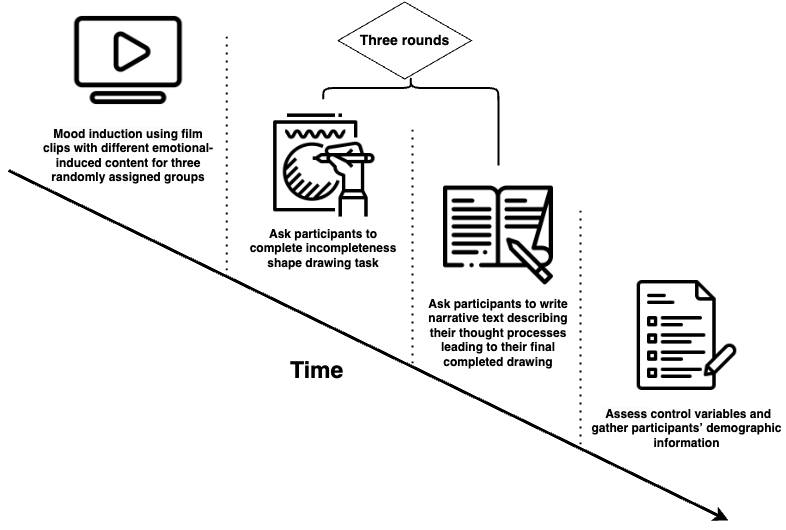
\includegraphics[height=0.8\textheight, keepaspectratio]{drawio/Experiment Timeline.png}
\end{figure}
\end{frame}

\begin{frame}{Mood Induction}
\begin{itemize}
    \item<1-> Films as effective mood induction techniques for engaging visual and auditory modalities and simulating real-life emotional situations (\cite{siedlecka_experimental_2019}).
    \item<2-> Select clips to induce happiness, calmness and neutral states based on emotional impacts (\cite{kucera_using_2012}).
    % \item<3-> Control display size and film duration and pre-screen participants who have viewed the films 
\end{itemize}
\end{frame}

\begin{frame}{Mood Induction}
\begin{itemize}
    \item<1-> Before experiment, participants will receive the instruction, “Please watch the film carefully,” to minimize framing effects on induced mood states.
    \item <2-> After experiment, check effectiveness of mood induction:
        \begin{enumerate}
            \item Rate the extent to which they are in a joyful, calm, or neural mood state when they watch the video.
            \item Rate the levels of valence (from unpleasant to pleasant) and arousal (from sleepy to highly aroused) of induced mood states (\cite{kucera_using_2012}).
        \end{enumerate}
\end{itemize}
\end{frame}


\begin{frame}{Implementing the Drawing Task}
Following \textcite{barbot_dynamics_2018}'s MTCI framework, this study will employ
\alert{incompleteness shape drawing task} to examine the visual creativity of participants, along with their creative processes (\cite{patterson_audra_2023}).

\begin{figure}
    \centering
    \includegraphics[height=0.45\textheight, keepaspectratio]{Weekly_assignments/Example of Incompleteness Shape Task.png}
    \caption{Example of Incompleteness Shape Task}
\end{figure}
\end{frame}

\begin{frame}{Implementing the Drawing Task}
Develop a web-based drawing interface using \href{https://www.jspsych.org/7.1/plugins/sketchpad/}{sketchpad} of jsPsych (\cite{leeuw_jspsych_2023}):
\begin{itemize}
    \item<1-> Include options for undoing, redoing, and clearing strokes.
    \item<2-> Record the position (x, y coordinates) and the timing of mouse movements during drawing.
    \item<3-> Save images as text (json-like structure) using base64 encoding for later data analysis (\cite{bainbridge_tutorial_2022}).
\end{itemize}

%Remember to add a screenshot of the web-based drawing interface!
% \begin{figure}
%     \centering
%     \includegraphics<4>[height=0.3\textheight]{Weekly_assignments/Example of Incompleteness Shape Task.png}
% \end{figure}
\end{frame}

% Flexibility (reliability and validity issues)
\begin{frame}{Operationalizing Flexibility Aspect of Creativity}
\begin{itemize}
    \item<1-> In the context of the incompleteness shape drawing task, flexibility hinges on participants' ability to \textbf{explore a wide range of qualitatively distinct creative solutions} (both in terms of starting position and trajectory) for each stroke they add to an incomplete shape. 
    \vspace{1em}
    \item<2-> This operational definition of flexibility assumes that a more creatively flexible individual will consider a broader array of potential next strokes and also be open to the possibility of choosing other paths qualitatively distinct from each other in their choice space during their creative processes. 
\end{itemize}
\end{frame}

\begin{frame}{Operationalizing Flexibility Aspect of Creativity}
\begin{itemize}
    \item \textbf{Compositional Stroke Embedding (CoSE) model} (\cite{aksan_cose_2021}) enables a novel perspective of examining the flexibility aspect of creativity by taking advantage of the model’s capability in next stroke prediction via Gaussian Mixture Model (GMM).
\end{itemize}
\end{frame}

\begin{frame}{Operationalizing Flexibility Aspect of Creativity}
\begin{figure}
    \centering
    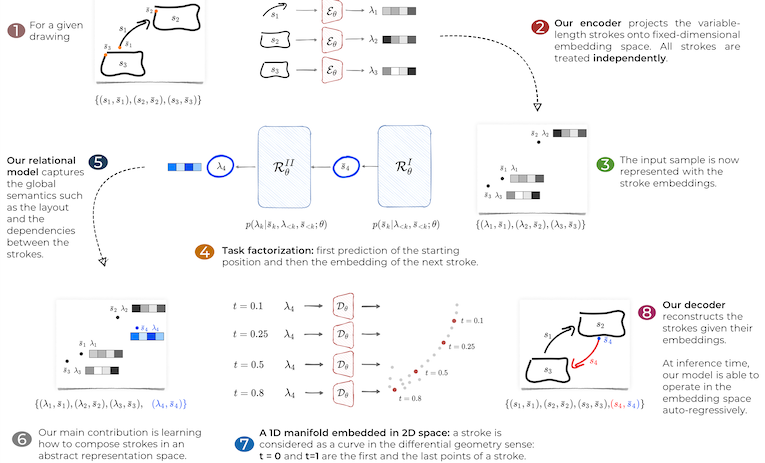
\includegraphics[height=0.75\textheight, keepaspectratio]{screenshots/CoSE Model Architecture.png}
    \caption{CoSE Model Architecture (\cite{aksan_cose_2021})}
\end{figure}
\end{frame}

\begin{frame}{Operationalizing Flexibility Aspect of Creativity}
\begin{itemize}
    \item<1-> The ability of CoSE to forecast strokes offers a tangible metric to assess the expansiveness and dynamic narrowing of creative possibilities: a) \textit{degrees of uncertainty (in its prediction)} and b) \textit{between-components (potential strokes) distances}.
    \vspace{1em}
    \item<2-> This proposed study will adopt 1) \alert{entropy of GMM} and 2) \alert{bhattacharyya distance} to capture degree of uncertainty and between-components distances in GMM’s prediction pertinent to the flexibility aspect of creative ideation process.
\end{itemize}
\end{frame}

\begin{frame}{Entropy of the Gaussian Mixture Model (GMM)}
\begin{itemize}
    \item<1-> Entropy measures the \alert{uncertainty} in the model's predictions for the next stroke. 
    \item<2-> High entropy indicates a state of high creative flexibility, where the participant is free to explore (and potentially follow) a wide range of directions for their next stroke at given number of completed strokes. 
    \item<3-> This proposed study utilizes \textcite{huber_entropy_2008}'s \alert{entropy approximation based on KL divergence}, which considers the diversity and weight of each component in the mixture, thus reflecting the variability and uncertainty in the model’s predictions for the next stroke in the drawing task.
\end{itemize}
\end{frame}

\begin{frame}{Bhattacharyya Distance $=>$ Component Divergence}
    \begin{itemize}
        \item<1-> Bhattacharyya Distance as a measure of divergence between two probability distributions.
        \item<1-> For GMM, assess the overlap and separation between different clusters (i.e., Gaussian components; \cite{alangari_intrinsically_2023}).
        \item<2-> Aggregated Bhattacharyya Distance in the context of GMM, where multiple Gaussian components represent different aspects of the data (creative possibilities), can be conceptualized as a measure of overall divergence or dissimilarity between all pairs of components within the model.
    \end{itemize}
\end{frame}

\begin{frame}{Bhattacharyya Distance $=>$ Component Divergence}
\begin{itemize}
    \item<1-> In the case of the incompleteness shape drawing task, the aggregated Bhattacharyya Distance across all component pairs in the GMM provides a quantitative measure of the \textbf{dynamic narrowing process of possibilities} of next stroke (positions and trajectories).
    \vspace{1em}
    \item<2-> A decrease in aggregated Bhattacharyya Distance over time indicates a gradual focusing of creative possibilities, reflecting participant’s transition from exploring a wide array of potential ideas to honing in on a more defined set of creative directions.
\end{itemize}
\end{frame}

\begin{frame}{Distinguishing Higher from Lower Flexibility in Creative Ideation Processes}
\begin{itemize}
    \item<1-> \alert{Average number}
        \begin{itemize}
            \item Broader, unpredictable exploration within the creative process
            \item Divergence in the exploration of creative possibilities, reflecting an engagement with a broad spectrum of cognitive categories.
        \end{itemize}
    \vspace{1em}
    \item<2-> \alert{Average rate of change}
        \begin{itemize}
            \item More extended period of ideational exploration (slower rate of convergence)
        \end{itemize}
    \vspace{1em}
    \item<3-> \alert{Number and timing of inflection points}
        \begin{itemize}
            \item A greater number of inflection points $=>$ A more dynamic process shifting between exploration and refinement
            \item Later occurrence of first major inflection point, marking the shift from initial exploration to more focused convergence
        \end{itemize}
\end{itemize}
\end{frame}

\begin{frame}{Operationalizing Flexibility Aspect of Creativity}
Apart from capturing the flexibility aspect of creativity using generative stroke models, this study relies on participants' \alert{verbal description on their thought processes} (behind their completed drawings) as a complementary measure to examine the diversity of ideas/concepts they connect during creative ideation processes. 
\end{frame}

\begin{frame}{Divergent Semantic Integration (DSI; \cite{johnson_divergent_2022})}
\begin{itemize}
    \item<1-> \textbf{Concept}: DSI measures the \textit{flexibility} aspect of creativity by assessing how narratives integrate divergent ideas, using the principle that semantic similarity is indicated by cooccurrence in text (\alert{distributional semantics theory}).
    \item<2-> \textbf{Computational Model}: 
        \begin{enumerate}
            \item Employs BERT to generate context-dependent embedding of words capturing nuanced semantic relationships that reflect creative integration;
            \item Calculates aggregated pairwise semantic distances to derive DSI scores - higher scores indicate a greater degree of creative divergence, and hence higher flexibility.
        \end{enumerate}
\end{itemize}
\end{frame}

% \begin{frame}{Divergent Semantic Integration (DSI; \cite{johnson_divergent_2022})}
% \begin{itemize}
%     \item \textbf{Application Methodology}:
%     \begin{itemize}
%         \begin{equation*}
%             DSI = \frac{2}{n(n-1)} \sum_{i=1}^{n} \sum_{k=i+1}^{n} D_{\text{cos}}(\omega_i, \omega_k)
%         \end{equation*}
%         \begin{equation*}
%             D_{\text{cos}}(\omega, k) = 1 - \frac{\omega \cdot k}{\|\omega\| \|k\|}
%         \end{equation*}
%         where:
%         \begin{itemize}
%             \item \(\omega_i, \omega_k\) are the embeddings for words \(i\) and \(k\).
%             \item \(D_{\text{cos}}\) measures the cosine distance, which is 1 minus the cosine similarity, between the embeddings.
%             \item \(n\) is the number of unique word pairs considered.
%         \end{itemize}
%     \end{itemize}
% \end{itemize}
% \end{frame}

\begin{frame}{Operationalizing Originality Aspect of Creativity}
Automated Drawing Assessment (\alert{AuDrA}; \cite{patterson_audra_2023}) is a model based on a modified ResNet architecture developed to assess the originality of sketches within the MTCI framework outlined by \textcite{barbot_dynamics_2018}:
\vspace{1em}
\begin{itemize}
    \item Trained over the same incompleteness shape drawing tasks.
    \item Trained with more than 13,000 sketches rated by nearly 60 human raters across four datasets.
\end{itemize}
\end{frame}

\begin{frame}
\frametitle{How AuDrA Enhances Creativity Research}
\begin{itemize}
    \item<1-> \textbf{Automated Originality Assessment:} A scalable and efficient method to assess the originality of creative outputs.
    \vspace{1em}
    \item<2-> \textbf{Integration with CoSE:} Complements other models like CoSE that assess different aspects of creativity, providing a comprehensive evaluation framework.
\end{itemize}
\end{frame}

\begin{frame}{Mediation Analysis}
\alert{Goal}: Explore how positive mood influences the originality aspect of creativity through the flexibility pathway.
% \begin{itemize}
%     \item<1-> \alert{Goal}: Explore how positive mood influences the originality aspect of creativity through the flexibility pathway.
%     % \item<2-> Multi-categorical mood conditions as independent variable (IV) $=>$ \textbf{Dummy coding} (\cite{hayes_statistical_2014}): 
%         % \begin{itemize}
%         %     \item<3-> To dummy-code \( k \) groups, \( k - 1 \) dummy variables are created.
%         %     \item<4-> Each dummy variable \( D_i \) (where \( i = 1, \ldots, k-1 \)) is set to 1 for cases in group \( i \), and 0 otherwise.
%         %     \item<5-> The unrepresented group (here, neural group) functions as the reference category.
%         % \end{itemize}
% \end{itemize}
\end{frame}

\begin{frame}{Model Setup}
    \begin{itemize}
        \item<1-> \textbf{Independent Variable (IV)}: Dummy-coded mood conditions (\cite{hayes_statistical_2014}):
        \begin{itemize}
            \item Happiness (D1)
            \item Calmness (D2)
            \item Neutral (Reference)
        \end{itemize}
        \item<2-> \textbf{Mediator (M)}: Flexibility in creativity
        \begin{itemize}
            \item Entropy \& bhattacharyya distance from drawing tasks
            \item DSI from after-drawing narrative
        \end{itemize}
        \item<3-> \textbf{Dependent Variable (DV)}: Output originality (from AuDrA)
        \item<4-> \textbf{Control Variables}: Cognitive abilities (intelligence, working memory, metacognitive ability) and self-rated artistic expertise
\end{itemize}
\end{frame}

% Preliminary Work Section
\section{Preliminary Work}
\begin{frame}{Building the Website}
 \href{https://www.kapwing.com/c/miV2nCSXYV}{This} is how I completed the website as a participant would. 
\begin{figure}
    \centering
    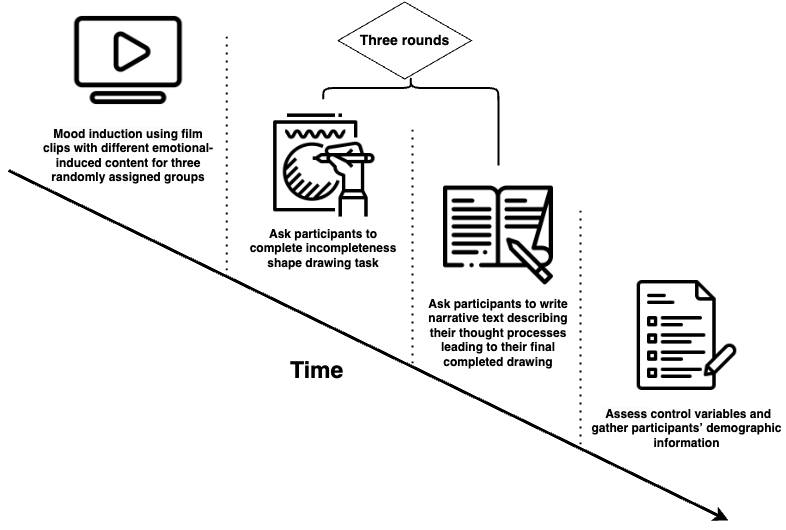
\includegraphics[height=0.6\textheight, keepaspectratio]{drawio/Experiment Timeline.png}
\end{figure}
% I first completed informed consent and then filled out some survey questions. Then, I watched a film clip for mood induction, before completing the incompleteness shape drawing task. After I finished drawing, I was asked to provide a label for my drawing, as well as a narrative on my thought processes leading to my final output. After completing the whole experiment, I could also see the result in json format, encompassing survey answers, completed drawings (including base64 encoding and coorindates), and narratives on thought processes.
\end{frame}

% Feasibility Assessment Section
\section{Feasibility Assessment}
% \begin{frame}{IRB approval}
% This proposed study is expected to receive IRB approval as it adheres to the four ethical principles (\cite{salganik_bit_2019}).
% \begin{itemize}
%     \item Respects the honor of participants by providing them with informed consent before the experiment. 
%     \item Maximizes potential benefits while minimizing potential harm to participants (as it does not induce negative emotions).
%     \item Treats every participant equally so that the benefits and risks are allocated fairly.
%     \item Complies with legal and public interest standards.
% \end{itemize}
% \end{frame}

\begin{frame}{Timeline}
\renewcommand{\arraystretch}{1.5}  % Adjusts the row height by a factor of 1.5
\begin{table}
\centering
\begin{tabular}{|l|p{7cm}|}
\hline
\textbf{Quarter} & \textbf{Activities} \\
\hline
Summer & Implement pilot study for pretesting. \\
\hline
Next autumn & 1) Refine experiment website and research design based on feedback from pilot study; \newline 2) Publish research design online and begin participant recruitment through MTurk. \\
\hline
Next winter & 1) Conduct data analysis; \newline 2) Complete the draft of the final thesis. \\
\hline
Next spring & Finalize and submit the thesis paper. \\
\hline
\end{tabular}
\end{table}
\end{frame}

% \begin{frame}{Costs}
% \begin{itemize}
%     \item Based on the pricing information provided on \href{https://requester.mturk.com/pricing}{Amazon Mechanical Turk website}, the total cost for each participant will be \$1.00 (base pay) + \$0.20 (MTurk fees) = \$1.20. 
%     \item For 300 participants, the total cost will be $\$1.20 \times 300 = \$360$.
% \end{itemize}
% \end{frame}

\begin{frame}{Deep Learning Models and Computing Power}
\begin{itemize}
    \item The pre-trained models and the running code for the two deep learning models I plan to use, i.e., \href{https://osf.io/kqn9v/}{AuDrA} and \href{https://github.com/eth-ait/cose}{CoSE} are publicly available online.
    \item This proposed study will utilize university high-performance computing clusters (specifically, Midway 3) for potential deep-learning model fine-tuning.
\end{itemize}
\end{frame}

\begin{frame}{Possible Advisors (Expert Support)}
\begin{columns}

% Column for Akram Bakkour
\begin{column}{0.5\textwidth}
\centering
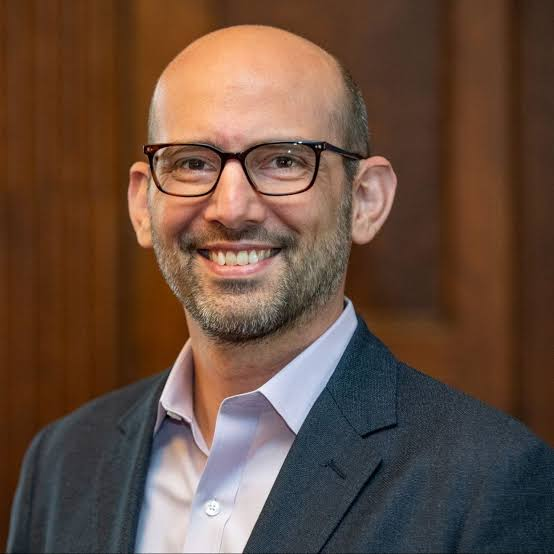
\includegraphics[width=0.8\linewidth]{screenshots/Akram Bakkour.png}\\
\textbf{Akram Bakkour} (UChicago)
\begin{itemize}
    \item Expert in cognitive psychology.
    \item Aids in research design and proposal drafting.
\end{itemize}
\end{column}

% Column for Roger Beaty
\begin{column}{0.5\textwidth}
\centering
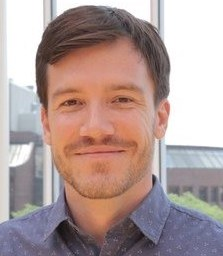
\includegraphics[width=0.8\linewidth]{screenshots/Roger Beaty.jpeg}\\
\textbf{Roger Beaty} (Penn State)
\begin{itemize}
    \item Expert in creativity and computational methods.
    \item Enriches research design and methodology.
\end{itemize}
\end{column}

\end{columns}
\end{frame}


% Ending section
% \section{Ending}
% \begin{frame}
% \begin{figure}
%     \centering
%     
\includegraphics[height=0.55\textheight, keepaspectratio]{screenshots/Repo QR Code.png}
%     \caption{QR code for the Github repository}
% \end{figure}
% \end{frame}

% Thanks for listenning
\begin{frame}
\begin{figure}
    \centering
    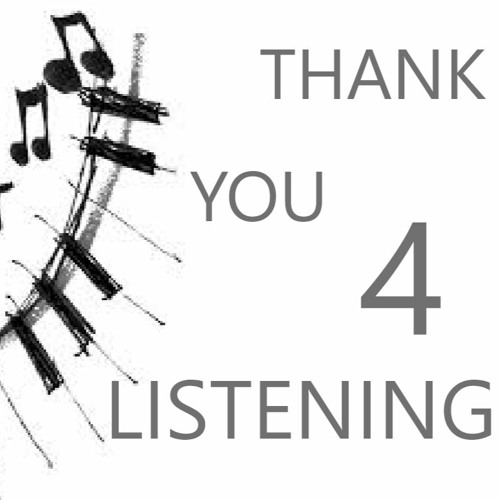
\includegraphics[width=0.8\linewidth]{screenshots/thanks_for_listening.jpeg}
\end{figure}
\end{frame}

% Appendix section for mediation analysis
\section{Appendix}
\begin{frame}{Formula of Entropy of GMM}
\begin{equation*}
    H(GMM) \approx -\sum_{i=1}^{N} \pi_i \log \left(\sum_{j=1}^{N} \pi_j \exp\left(-\frac{1}{2} D_{KL}(N_i || N_j)\right)\right),
\end{equation*}
\begin{equation*}
    \begin{split}
    D_{KL}(N_i || N_j) = \frac{1}{2} \bigg( \text{tr}(\Sigma_j^{-1}\Sigma_i) + (\mu_j - \mu_i)^T \Sigma_j^{-1} (\mu_j - \mu_i) - k \\
    + \ln\left(\frac{|\Sigma_j|}{|\Sigma_i|}\right) \bigg),
\end{split}
\end{equation*}

\begin{itemize}
    \item \(N\) is the number of components in the GMM.
    \item \(\pi_i\), \(\pi_j\) are the mixing coefficients.
    \item \(D_{KL}(N_i || N_j)\) is the KL divergence between components.
    \item \(\Sigma_i\), \(\Sigma_j\) are the covariance matrices.
    \item \(\mu_i\), \(\mu_j\) are the mean vectors.
    \item \(\text{tr}(\cdot)\) is the trace of a matrix.
    \item \(k\) is the dimensionality of the data.
    \item \(|\Sigma|\) is the determinant of the covariance matrix.
\end{itemize}
\end{frame}

\begin{frame}{Formula of Bhattacharyya Distance}
Given a GMM with $N$ components, each defined by a mean vector $\mu_i$ and a covariance matrix $\Sigma_i$: 
    \begin{itemize}
        \item \textbf{Bhattacharyya Distance (BD) between any two components $i$ and $j$} can be calculated as:
            \begin{equation*}
                BD[\mu_i, \Sigma_i, \mu_j, \Sigma_j] = \frac{1}{8} \Delta\mu_{ij}^T \left(\frac{\Sigma_i + \Sigma_j}{2}\right)^{-1} \Delta\mu_{ij} + \frac{1}{2} \ln \left(\frac{|\frac{\Sigma_i + \Sigma_j}{2}|}{\sqrt{|\Sigma_i||\Sigma_j|}}\right)
            \end{equation*}
            where \(\Delta\mu_{ij} = \mu_j - \mu_i\) is the difference between the mean vectors of components \(i\) and \(j\)
        \item \textbf{Aggregated Bhattacharyya Distance} (averaged all unique pairs of GMM components):
            \begin{equation*}
                DAB = \frac{1}{\binom{N}{2}} \sum_{i=1}^{N} \sum_{j=i+1}^{N} BC[\mu_i, \Sigma_i, \mu_j, \Sigma_j]
            \end{equation*}
    \end{itemize}
\end{frame}

\begin{frame}{Formula of Divergent Semantic Integration}
\begin{equation*}
    DSI = \frac{2}{n(n-1)} \sum_{i=1}^{n} \sum_{k=i+1}^{n} D_{\text{cos}}(\omega_i, \omega_k)
\end{equation*}
\begin{equation*}
    D_{\text{cos}}(\omega, k) = 1 - \frac{\omega \cdot k}{\|\omega\| \|k\|}
\end{equation*}
where:
\begin{itemize}
    \item \(\omega_i, \omega_k\) are the embeddings for words \(i\) and \(k\).
    \item \(D_{\text{cos}}\) measures the cosine distance, which is 1 minus the cosine similarity, between the embeddings.
    \item \(n\) is the number of unique word pairs considered.
\end{itemize}
\end{frame}

\begin{frame}{Mediation Model Representation}
\begin{itemize}
    \item Mediator Model:
    \[ M = \alpha_0 + \alpha_1 D1 + \alpha_2 D2 + \alpha_3 X + \epsilon_M \]
    \begin{itemize}
        \item \( M \) - Mediator variable (flexibility in creativity)
        \item \( \alpha_0 \) - Intercept of the mediator model
        \item \( \alpha_1, \alpha_2 \) - Coefficients for the effect of mood conditions (Happiness and Calmness) on \( M \)
        \item \( D1, D2 \) - Dummy variables for mood conditions: \( D1 \) for Happiness, \( D2 \) for Calmness
        \item \( X \) - Vector of control variables (e.g., cognitive abilities, artistic expertise)
        \item \( \alpha_3 \) - Vector of coefficients for control variables in the mediator model
        \item \( \epsilon_M \) - Error term for the mediator model
    \end{itemize}
\end{itemize}
\end{frame}

\begin{frame}{Mediation Model Representation}
\begin{itemize}
\item Outcome Model:
    \[ Y = \beta_0 + \beta_1 D1 + \beta_2 D2 + \beta_3 M + \beta_4 X + \epsilon_Y \]
    \begin{itemize}
        \item \( Y \) - Dependent variable (originality in creativity)
        \item \( \beta_0 \) - Intercept of the outcome model
        \item \( \beta_1, \beta_2 \) - Coefficients for the direct effects of mood conditions on \( Y \)
        \item \( \beta_3 \) - Coefficient for the effect of \( M \) on \( Y \)
        \item \( \beta_4 \) - Vector of coefficients for control variables in the outcome model
        \item \( \epsilon_Y \) - Error term for the outcome model
    \end{itemize}
\end{itemize}
\end{frame}

\begin{frame}{Interpretation of Effects}
\begin{itemize}
    \item \textbf{Indirect Effects} ($aib$):
    \begin{itemize}
        \item Represent the product of the coefficients from mood to flexibility ($\alpha_1, \alpha_2$) and from flexibility to originality ($\beta_3$).
        \item Formula for Happiness: $\alpha_1 \times \beta_3$
        \item Formula for Calmness: $\alpha_2 \times \beta_3$
    \end{itemize}
    \item \textbf{Direct Effects} ($c'_{i}$):
    \begin{itemize}
        \item Measured by the coefficients ($\beta_1, \beta_2$) which represent the impact of each mood condition directly on originality, not through flexibility.
        \item Formula for Happiness: $\beta_1$
        \item Formula for Calmness: $\beta_2$
    \end{itemize}
    \item \textbf{Total Effects}:
    \begin{itemize}
        \item Sum of the direct and indirect effects for each mood condition.
        \item Formula for Happiness: $\beta_1 + (\alpha_1 \times \beta_3)$
        \item Formula for Calmness: $\beta_2 + (\alpha_2 \times \beta_3)$
    \end{itemize}
\end{itemize}
\end{frame}

\end{document}
